% Created by tikzDevice version 0.12.6 on 2026-08-01 04:31:26
% !TEX encoding = UTF-8 Unicode
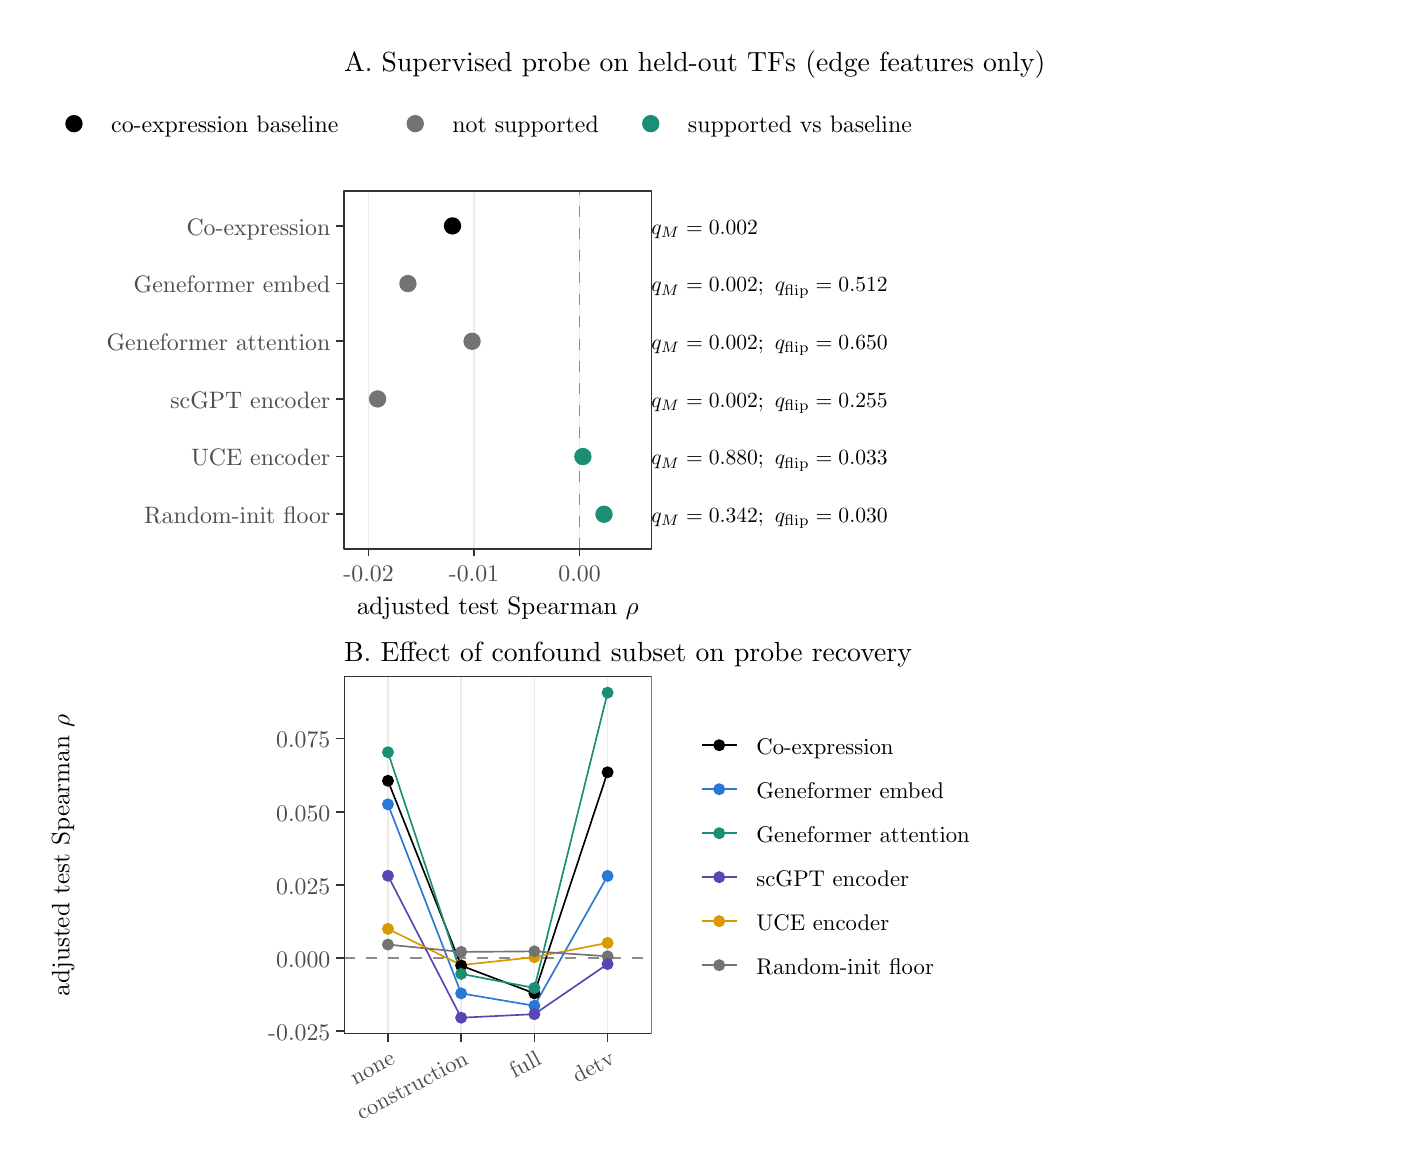
\begin{tikzpicture}[x=1pt,y=1pt]
\definecolor{fillColor}{RGB}{255,255,255}
\path[use as bounding box,fill=fillColor,fill opacity=0.00] (0,0) rectangle (491.44,404.71);
\begin{scope}
\path[clip] (  0.00,  0.00) rectangle (491.44,404.71);
\definecolor{drawColor}{RGB}{255,255,255}
\definecolor{fillColor}{RGB}{255,255,255}

\path[draw=drawColor,line width= 0.6pt,line join=round,line cap=round,fill=fillColor] (  0.00,  0.00) rectangle (491.44,404.71);
\end{scope}
\begin{scope}
\path[clip] (  4.00,187.52) rectangle (485.44,400.71);
\definecolor{drawColor}{RGB}{255,255,255}
\definecolor{fillColor}{RGB}{255,255,255}

\path[draw=drawColor,line width= 0.6pt,line join=round,line cap=round,fill=fillColor] (  4.00,187.52) rectangle (485.44,400.71);
\end{scope}
\begin{scope}
\path[clip] (  4.00,  3.00) rectangle (485.44,187.52);
\definecolor{drawColor}{RGB}{255,255,255}
\definecolor{fillColor}{RGB}{255,255,255}

\path[draw=drawColor,line width= 0.6pt,line join=round,line cap=round,fill=fillColor] (  4.00,  3.00) rectangle (485.44,187.52);
\end{scope}
\begin{scope}
\path[clip] (  0.00,  0.00) rectangle (491.44,404.71);
\definecolor{fillColor}{RGB}{255,255,255}

\path[fill=fillColor] (114.31,216.37) rectangle (225.43,345.57);
\definecolor{drawColor}{gray}{0.92}

\path[draw=drawColor,line width= 0.6pt,line join=round] (123.18,216.37) --
	(123.18,345.57);

\path[draw=drawColor,line width= 0.6pt,line join=round] (161.29,216.37) --
	(161.29,345.57);

\path[draw=drawColor,line width= 0.6pt,line join=round] (199.41,216.37) --
	(199.41,345.57);
\definecolor{drawColor}{gray}{0.55}

\path[draw=drawColor,line width= 0.6pt,dash pattern=on 4pt off 4pt ,line join=round] (199.41,216.37) -- (199.41,345.57);
\definecolor{drawColor}{RGB}{27,143,117}
\definecolor{fillColor}{RGB}{27,143,117}

\path[draw=drawColor,line width= 0.4pt,line join=round,line cap=round,fill=fillColor] (200.62,249.72) circle (  2.93);
\definecolor{drawColor}{RGB}{0,0,0}
\definecolor{fillColor}{RGB}{0,0,0}

\path[draw=drawColor,line width= 0.4pt,line join=round,line cap=round,fill=fillColor] (153.51,333.07) circle (  2.93);
\definecolor{drawColor}{gray}{0.45}
\definecolor{fillColor}{gray}{0.45}

\path[draw=drawColor,line width= 0.4pt,line join=round,line cap=round,fill=fillColor] (160.58,291.39) circle (  2.93);

\path[draw=drawColor,line width= 0.4pt,line join=round,line cap=round,fill=fillColor] (137.40,312.23) circle (  2.93);
\definecolor{drawColor}{RGB}{27,143,117}
\definecolor{fillColor}{RGB}{27,143,117}

\path[draw=drawColor,line width= 0.4pt,line join=round,line cap=round,fill=fillColor] (208.25,228.88) circle (  2.93);
\definecolor{drawColor}{gray}{0.45}
\definecolor{fillColor}{gray}{0.45}

\path[draw=drawColor,line width= 0.4pt,line join=round,line cap=round,fill=fillColor] (126.44,270.55) circle (  2.93);
\definecolor{drawColor}{RGB}{0,0,0}

\node[text=drawColor,anchor=base west,inner sep=0pt, outer sep=0pt, scale=  0.78] at (225.33,246.69) {$q_M=0.880;\ q_{\mathrm{flip}}=0.033$};

\node[text=drawColor,anchor=base west,inner sep=0pt, outer sep=0pt, scale=  0.78] at (225.33,330.04) {$q_M=0.002$};

\node[text=drawColor,anchor=base west,inner sep=0pt, outer sep=0pt, scale=  0.78] at (225.33,288.37) {$q_M=0.002;\ q_{\mathrm{flip}}=0.650$};

\node[text=drawColor,anchor=base west,inner sep=0pt, outer sep=0pt, scale=  0.78] at (225.33,309.21) {$q_M=0.002;\ q_{\mathrm{flip}}=0.512$};

\node[text=drawColor,anchor=base west,inner sep=0pt, outer sep=0pt, scale=  0.78] at (225.33,225.85) {$q_M=0.342;\ q_{\mathrm{flip}}=0.030$};

\node[text=drawColor,anchor=base west,inner sep=0pt, outer sep=0pt, scale=  0.78] at (225.33,267.53) {$q_M=0.002;\ q_{\mathrm{flip}}=0.255$};
\definecolor{drawColor}{gray}{0.20}

\path[draw=drawColor,line width= 0.6pt,line join=round,line cap=round] (114.31,216.37) rectangle (225.43,345.57);
\end{scope}
\begin{scope}
\path[clip] (  0.00,  0.00) rectangle (491.44,404.71);
\definecolor{drawColor}{gray}{0.30}

\node[text=drawColor,anchor=base east,inner sep=0pt, outer sep=0pt, scale=  0.86] at (109.36,225.51) {Random-init floor};

\node[text=drawColor,anchor=base east,inner sep=0pt, outer sep=0pt, scale=  0.86] at (109.36,246.35) {UCE encoder};

\node[text=drawColor,anchor=base east,inner sep=0pt, outer sep=0pt, scale=  0.86] at (109.36,267.19) {scGPT encoder};

\node[text=drawColor,anchor=base east,inner sep=0pt, outer sep=0pt, scale=  0.86] at (109.36,288.02) {Geneformer attention};

\node[text=drawColor,anchor=base east,inner sep=0pt, outer sep=0pt, scale=  0.86] at (109.36,308.86) {Geneformer embed};

\node[text=drawColor,anchor=base east,inner sep=0pt, outer sep=0pt, scale=  0.86] at (109.36,329.70) {Co-expression};
\end{scope}
\begin{scope}
\path[clip] (  0.00,  0.00) rectangle (491.44,404.71);
\definecolor{drawColor}{gray}{0.20}

\path[draw=drawColor,line width= 0.6pt,line join=round] (111.56,228.88) --
	(114.31,228.88);

\path[draw=drawColor,line width= 0.6pt,line join=round] (111.56,249.72) --
	(114.31,249.72);

\path[draw=drawColor,line width= 0.6pt,line join=round] (111.56,270.55) --
	(114.31,270.55);

\path[draw=drawColor,line width= 0.6pt,line join=round] (111.56,291.39) --
	(114.31,291.39);

\path[draw=drawColor,line width= 0.6pt,line join=round] (111.56,312.23) --
	(114.31,312.23);

\path[draw=drawColor,line width= 0.6pt,line join=round] (111.56,333.07) --
	(114.31,333.07);
\end{scope}
\begin{scope}
\path[clip] (  0.00,  0.00) rectangle (491.44,404.71);
\definecolor{drawColor}{gray}{0.20}

\path[draw=drawColor,line width= 0.6pt,line join=round] (123.18,213.62) --
	(123.18,216.37);

\path[draw=drawColor,line width= 0.6pt,line join=round] (161.29,213.62) --
	(161.29,216.37);

\path[draw=drawColor,line width= 0.6pt,line join=round] (199.41,213.62) --
	(199.41,216.37);
\end{scope}
\begin{scope}
\path[clip] (  0.00,  0.00) rectangle (491.44,404.71);
\definecolor{drawColor}{gray}{0.30}

\node[text=drawColor,anchor=base,inner sep=0pt, outer sep=0pt, scale=  0.86] at (123.18,204.69) {-0.02};

\node[text=drawColor,anchor=base,inner sep=0pt, outer sep=0pt, scale=  0.86] at (161.29,204.69) {-0.01};

\node[text=drawColor,anchor=base,inner sep=0pt, outer sep=0pt, scale=  0.86] at (199.41,204.69) {0.00};
\end{scope}
\begin{scope}
\path[clip] (  0.00,  0.00) rectangle (491.44,404.71);
\definecolor{drawColor}{RGB}{0,0,0}

\node[text=drawColor,anchor=base,inner sep=0pt, outer sep=0pt, scale=  0.91] at (169.87,192.74) {adjusted test Spearman $\rho$};
\end{scope}
\begin{scope}
\path[clip] (  0.00,  0.00) rectangle (491.44,404.71);
\definecolor{fillColor}{RGB}{255,255,255}

\path[fill=fillColor] (  3.28,356.57) rectangle (336.46,383.47);
\end{scope}
\begin{scope}
\path[clip] (  0.00,  0.00) rectangle (491.44,404.71);
\definecolor{fillColor}{RGB}{255,255,255}

\path[fill=fillColor] (  8.78,362.07) rectangle ( 24.68,377.97);
\definecolor{drawColor}{RGB}{0,0,0}
\definecolor{fillColor}{RGB}{0,0,0}

\path[draw=drawColor,line width= 0.4pt,line join=round,line cap=round,fill=fillColor] ( 16.73,370.02) circle (  2.93);
\end{scope}
\begin{scope}
\path[clip] (  0.00,  0.00) rectangle (491.44,404.71);
\definecolor{fillColor}{RGB}{255,255,255}

\path[fill=fillColor] (132.10,362.07) rectangle (148.00,377.97);
\definecolor{drawColor}{gray}{0.45}
\definecolor{fillColor}{gray}{0.45}

\path[draw=drawColor,line width= 0.4pt,line join=round,line cap=round,fill=fillColor] (140.05,370.02) circle (  2.93);
\end{scope}
\begin{scope}
\path[clip] (  0.00,  0.00) rectangle (491.44,404.71);
\definecolor{fillColor}{RGB}{255,255,255}

\path[fill=fillColor] (217.20,362.07) rectangle (233.10,377.97);
\definecolor{drawColor}{RGB}{27,143,117}
\definecolor{fillColor}{RGB}{27,143,117}

\path[draw=drawColor,line width= 0.4pt,line join=round,line cap=round,fill=fillColor] (225.15,370.02) circle (  2.93);
\end{scope}
\begin{scope}
\path[clip] (  0.00,  0.00) rectangle (491.44,404.71);
\definecolor{drawColor}{RGB}{0,0,0}

\node[text=drawColor,anchor=base west,inner sep=0pt, outer sep=0pt, scale=  0.86] at ( 30.18,366.66) {co-expression baseline};
\end{scope}
\begin{scope}
\path[clip] (  0.00,  0.00) rectangle (491.44,404.71);
\definecolor{drawColor}{RGB}{0,0,0}

\node[text=drawColor,anchor=base west,inner sep=0pt, outer sep=0pt, scale=  0.86] at (153.50,366.66) {not supported};
\end{scope}
\begin{scope}
\path[clip] (  0.00,  0.00) rectangle (491.44,404.71);
\definecolor{drawColor}{RGB}{0,0,0}

\node[text=drawColor,anchor=base west,inner sep=0pt, outer sep=0pt, scale=  0.86] at (238.60,366.66) {supported vs baseline};
\end{scope}
\begin{scope}
\path[clip] (  0.00,  0.00) rectangle (491.44,404.71);
\definecolor{drawColor}{RGB}{0,0,0}

\node[text=drawColor,anchor=base west,inner sep=0pt, outer sep=0pt, scale=  1.00] at (114.31,388.91) {A. Supervised probe on held-out TFs (edge features only)};
\end{scope}
\begin{scope}
\path[clip] (114.31, 41.08) rectangle (225.43,170.29);
\definecolor{fillColor}{RGB}{255,255,255}

\path[fill=fillColor] (114.31, 41.08) rectangle (225.43,170.29);
\definecolor{drawColor}{gray}{0.92}

\path[draw=drawColor,line width= 0.6pt,line join=round] (130.19, 41.08) --
	(130.19,170.29);

\path[draw=drawColor,line width= 0.6pt,line join=round] (156.64, 41.08) --
	(156.64,170.29);

\path[draw=drawColor,line width= 0.6pt,line join=round] (183.10, 41.08) --
	(183.10,170.29);

\path[draw=drawColor,line width= 0.6pt,line join=round] (209.55, 41.08) --
	(209.55,170.29);
\definecolor{drawColor}{gray}{0.55}

\path[draw=drawColor,line width= 0.6pt,dash pattern=on 4pt off 4pt ,line join=round] (114.31, 68.49) -- (225.43, 68.49);
\definecolor{drawColor}{RGB}{0,0,0}

\path[draw=drawColor,line width= 0.6pt,line join=round] (130.19,132.57) --
	(156.64, 65.78) --
	(183.10, 55.75) --
	(209.55,135.65);
\definecolor{drawColor}{RGB}{42,120,214}

\path[draw=drawColor,line width= 0.6pt,line join=round] (130.19,124.06) --
	(156.64, 55.75) --
	(183.10, 51.28) --
	(209.55, 98.18);
\definecolor{drawColor}{RGB}{27,143,117}

\path[draw=drawColor,line width= 0.6pt,line join=round] (130.19,142.90) --
	(156.64, 62.80) --
	(183.10, 57.71) --
	(209.55,164.41);
\definecolor{drawColor}{RGB}{89,70,178}

\path[draw=drawColor,line width= 0.6pt,line join=round] (130.19, 98.26) --
	(156.64, 46.96) --
	(183.10, 48.24) --
	(209.55, 66.35);
\definecolor{drawColor}{RGB}{217,154,0}

\path[draw=drawColor,line width= 0.6pt,line join=round] (130.19, 79.06) --
	(156.64, 65.98) --
	(183.10, 68.83) --
	(209.55, 74.00);
\definecolor{drawColor}{gray}{0.45}

\path[draw=drawColor,line width= 0.6pt,line join=round] (130.19, 73.39) --
	(156.64, 70.73) --
	(183.10, 70.94) --
	(209.55, 69.15);
\definecolor{drawColor}{RGB}{217,154,0}
\definecolor{fillColor}{RGB}{217,154,0}

\path[draw=drawColor,line width= 0.4pt,line join=round,line cap=round,fill=fillColor] (156.64, 65.98) circle (  1.96);

\path[draw=drawColor,line width= 0.4pt,line join=round,line cap=round,fill=fillColor] (209.55, 74.00) circle (  1.96);

\path[draw=drawColor,line width= 0.4pt,line join=round,line cap=round,fill=fillColor] (183.10, 68.83) circle (  1.96);

\path[draw=drawColor,line width= 0.4pt,line join=round,line cap=round,fill=fillColor] (130.19, 79.06) circle (  1.96);
\definecolor{drawColor}{RGB}{0,0,0}
\definecolor{fillColor}{RGB}{0,0,0}

\path[draw=drawColor,line width= 0.4pt,line join=round,line cap=round,fill=fillColor] (156.64, 65.78) circle (  1.96);

\path[draw=drawColor,line width= 0.4pt,line join=round,line cap=round,fill=fillColor] (209.55,135.65) circle (  1.96);

\path[draw=drawColor,line width= 0.4pt,line join=round,line cap=round,fill=fillColor] (183.10, 55.75) circle (  1.96);

\path[draw=drawColor,line width= 0.4pt,line join=round,line cap=round,fill=fillColor] (130.19,132.57) circle (  1.96);
\definecolor{drawColor}{RGB}{27,143,117}
\definecolor{fillColor}{RGB}{27,143,117}

\path[draw=drawColor,line width= 0.4pt,line join=round,line cap=round,fill=fillColor] (156.64, 62.80) circle (  1.96);

\path[draw=drawColor,line width= 0.4pt,line join=round,line cap=round,fill=fillColor] (209.55,164.41) circle (  1.96);

\path[draw=drawColor,line width= 0.4pt,line join=round,line cap=round,fill=fillColor] (183.10, 57.71) circle (  1.96);

\path[draw=drawColor,line width= 0.4pt,line join=round,line cap=round,fill=fillColor] (130.19,142.90) circle (  1.96);
\definecolor{drawColor}{RGB}{42,120,214}
\definecolor{fillColor}{RGB}{42,120,214}

\path[draw=drawColor,line width= 0.4pt,line join=round,line cap=round,fill=fillColor] (156.64, 55.75) circle (  1.96);

\path[draw=drawColor,line width= 0.4pt,line join=round,line cap=round,fill=fillColor] (209.55, 98.18) circle (  1.96);

\path[draw=drawColor,line width= 0.4pt,line join=round,line cap=round,fill=fillColor] (183.10, 51.28) circle (  1.96);

\path[draw=drawColor,line width= 0.4pt,line join=round,line cap=round,fill=fillColor] (130.19,124.06) circle (  1.96);
\definecolor{drawColor}{gray}{0.45}
\definecolor{fillColor}{gray}{0.45}

\path[draw=drawColor,line width= 0.4pt,line join=round,line cap=round,fill=fillColor] (156.64, 70.73) circle (  1.96);

\path[draw=drawColor,line width= 0.4pt,line join=round,line cap=round,fill=fillColor] (209.55, 69.15) circle (  1.96);

\path[draw=drawColor,line width= 0.4pt,line join=round,line cap=round,fill=fillColor] (183.10, 70.94) circle (  1.96);

\path[draw=drawColor,line width= 0.4pt,line join=round,line cap=round,fill=fillColor] (130.19, 73.39) circle (  1.96);
\definecolor{drawColor}{RGB}{89,70,178}
\definecolor{fillColor}{RGB}{89,70,178}

\path[draw=drawColor,line width= 0.4pt,line join=round,line cap=round,fill=fillColor] (156.64, 46.96) circle (  1.96);

\path[draw=drawColor,line width= 0.4pt,line join=round,line cap=round,fill=fillColor] (209.55, 66.35) circle (  1.96);

\path[draw=drawColor,line width= 0.4pt,line join=round,line cap=round,fill=fillColor] (183.10, 48.24) circle (  1.96);

\path[draw=drawColor,line width= 0.4pt,line join=round,line cap=round,fill=fillColor] (130.19, 98.26) circle (  1.96);
\definecolor{drawColor}{gray}{0.20}

\path[draw=drawColor,line width= 0.6pt,line join=round,line cap=round] (114.31, 41.08) rectangle (225.43,170.29);
\end{scope}
\begin{scope}
\path[clip] (  0.00,  0.00) rectangle (491.44,404.71);
\definecolor{drawColor}{gray}{0.30}

\node[text=drawColor,anchor=base east,inner sep=0pt, outer sep=0pt, scale=  0.86] at (109.36, 38.68) {-0.025};

\node[text=drawColor,anchor=base east,inner sep=0pt, outer sep=0pt, scale=  0.86] at (109.36, 65.12) {0.000};

\node[text=drawColor,anchor=base east,inner sep=0pt, outer sep=0pt, scale=  0.86] at (109.36, 91.56) {0.025};

\node[text=drawColor,anchor=base east,inner sep=0pt, outer sep=0pt, scale=  0.86] at (109.36,118.00) {0.050};

\node[text=drawColor,anchor=base east,inner sep=0pt, outer sep=0pt, scale=  0.86] at (109.36,144.44) {0.075};
\end{scope}
\begin{scope}
\path[clip] (  0.00,  0.00) rectangle (491.44,404.71);
\definecolor{drawColor}{gray}{0.20}

\path[draw=drawColor,line width= 0.6pt,line join=round] (111.56, 42.05) --
	(114.31, 42.05);

\path[draw=drawColor,line width= 0.6pt,line join=round] (111.56, 68.49) --
	(114.31, 68.49);

\path[draw=drawColor,line width= 0.6pt,line join=round] (111.56, 94.93) --
	(114.31, 94.93);

\path[draw=drawColor,line width= 0.6pt,line join=round] (111.56,121.37) --
	(114.31,121.37);

\path[draw=drawColor,line width= 0.6pt,line join=round] (111.56,147.81) --
	(114.31,147.81);
\end{scope}
\begin{scope}
\path[clip] (  0.00,  0.00) rectangle (491.44,404.71);
\definecolor{drawColor}{gray}{0.20}

\path[draw=drawColor,line width= 0.6pt,line join=round] (130.19, 38.33) --
	(130.19, 41.08);

\path[draw=drawColor,line width= 0.6pt,line join=round] (156.64, 38.33) --
	(156.64, 41.08);

\path[draw=drawColor,line width= 0.6pt,line join=round] (183.10, 38.33) --
	(183.10, 41.08);

\path[draw=drawColor,line width= 0.6pt,line join=round] (209.55, 38.33) --
	(209.55, 41.08);
\end{scope}
\begin{scope}
\path[clip] (  0.00,  0.00) rectangle (491.44,404.71);
\definecolor{drawColor}{gray}{0.30}

\node[text=drawColor,rotate= 28.00,anchor=base east,inner sep=0pt, outer sep=0pt, scale=  0.82] at (133.18, 30.50) {none};

\node[text=drawColor,rotate= 28.00,anchor=base east,inner sep=0pt, outer sep=0pt, scale=  0.82] at (159.64, 30.50) {construction};

\node[text=drawColor,rotate= 28.00,anchor=base east,inner sep=0pt, outer sep=0pt, scale=  0.82] at (186.09, 30.50) {full};

\node[text=drawColor,rotate= 28.00,anchor=base east,inner sep=0pt, outer sep=0pt, scale=  0.82] at (212.55, 30.50) {detv};
\end{scope}
\begin{scope}
\path[clip] (  0.00,  0.00) rectangle (491.44,404.71);
\definecolor{drawColor}{RGB}{0,0,0}

\node[text=drawColor,rotate= 90.00,anchor=base,inner sep=0pt, outer sep=0pt, scale=  0.91] at ( 15.09,105.69) {adjusted test Spearman $\rho$};
\end{scope}
\begin{scope}
\path[clip] (  0.00,  0.00) rectangle (491.44,404.71);
\definecolor{fillColor}{RGB}{255,255,255}

\path[fill=fillColor] (236.43, 52.49) rectangle (353.44,158.88);
\end{scope}
\begin{scope}
\path[clip] (  0.00,  0.00) rectangle (491.44,404.71);
\definecolor{fillColor}{RGB}{255,255,255}

\path[fill=fillColor] (241.93,137.48) rectangle (257.83,153.38);
\definecolor{drawColor}{RGB}{0,0,0}

\path[draw=drawColor,line width= 0.6pt,line join=round] (243.52,145.43) -- (256.24,145.43);
\definecolor{fillColor}{RGB}{0,0,0}

\path[draw=drawColor,line width= 0.4pt,line join=round,line cap=round,fill=fillColor] (249.88,145.43) circle (  1.96);
\end{scope}
\begin{scope}
\path[clip] (  0.00,  0.00) rectangle (491.44,404.71);
\definecolor{fillColor}{RGB}{255,255,255}

\path[fill=fillColor] (241.93,121.58) rectangle (257.83,137.48);
\definecolor{drawColor}{RGB}{42,120,214}

\path[draw=drawColor,line width= 0.6pt,line join=round] (243.52,129.53) -- (256.24,129.53);
\definecolor{fillColor}{RGB}{42,120,214}

\path[draw=drawColor,line width= 0.4pt,line join=round,line cap=round,fill=fillColor] (249.88,129.53) circle (  1.96);
\end{scope}
\begin{scope}
\path[clip] (  0.00,  0.00) rectangle (491.44,404.71);
\definecolor{fillColor}{RGB}{255,255,255}

\path[fill=fillColor] (241.93,105.69) rectangle (257.83,121.58);
\definecolor{drawColor}{RGB}{27,143,117}

\path[draw=drawColor,line width= 0.6pt,line join=round] (243.52,113.63) -- (256.24,113.63);
\definecolor{fillColor}{RGB}{27,143,117}

\path[draw=drawColor,line width= 0.4pt,line join=round,line cap=round,fill=fillColor] (249.88,113.63) circle (  1.96);
\end{scope}
\begin{scope}
\path[clip] (  0.00,  0.00) rectangle (491.44,404.71);
\definecolor{fillColor}{RGB}{255,255,255}

\path[fill=fillColor] (241.93, 89.79) rectangle (257.83,105.69);
\definecolor{drawColor}{RGB}{89,70,178}

\path[draw=drawColor,line width= 0.6pt,line join=round] (243.52, 97.74) -- (256.24, 97.74);
\definecolor{fillColor}{RGB}{89,70,178}

\path[draw=drawColor,line width= 0.4pt,line join=round,line cap=round,fill=fillColor] (249.88, 97.74) circle (  1.96);
\end{scope}
\begin{scope}
\path[clip] (  0.00,  0.00) rectangle (491.44,404.71);
\definecolor{fillColor}{RGB}{255,255,255}

\path[fill=fillColor] (241.93, 73.89) rectangle (257.83, 89.79);
\definecolor{drawColor}{RGB}{217,154,0}

\path[draw=drawColor,line width= 0.6pt,line join=round] (243.52, 81.84) -- (256.24, 81.84);
\definecolor{fillColor}{RGB}{217,154,0}

\path[draw=drawColor,line width= 0.4pt,line join=round,line cap=round,fill=fillColor] (249.88, 81.84) circle (  1.96);
\end{scope}
\begin{scope}
\path[clip] (  0.00,  0.00) rectangle (491.44,404.71);
\definecolor{fillColor}{RGB}{255,255,255}

\path[fill=fillColor] (241.93, 57.99) rectangle (257.83, 73.89);
\definecolor{drawColor}{gray}{0.45}

\path[draw=drawColor,line width= 0.6pt,line join=round] (243.52, 65.94) -- (256.24, 65.94);
\definecolor{fillColor}{gray}{0.45}

\path[draw=drawColor,line width= 0.4pt,line join=round,line cap=round,fill=fillColor] (249.88, 65.94) circle (  1.96);
\end{scope}
\begin{scope}
\path[clip] (  0.00,  0.00) rectangle (491.44,404.71);
\definecolor{drawColor}{RGB}{0,0,0}

\node[text=drawColor,anchor=base west,inner sep=0pt, outer sep=0pt, scale=  0.82] at (263.33,142.24) {Co-expression};
\end{scope}
\begin{scope}
\path[clip] (  0.00,  0.00) rectangle (491.44,404.71);
\definecolor{drawColor}{RGB}{0,0,0}

\node[text=drawColor,anchor=base west,inner sep=0pt, outer sep=0pt, scale=  0.82] at (263.33,126.34) {Geneformer embed};
\end{scope}
\begin{scope}
\path[clip] (  0.00,  0.00) rectangle (491.44,404.71);
\definecolor{drawColor}{RGB}{0,0,0}

\node[text=drawColor,anchor=base west,inner sep=0pt, outer sep=0pt, scale=  0.82] at (263.33,110.44) {Geneformer attention};
\end{scope}
\begin{scope}
\path[clip] (  0.00,  0.00) rectangle (491.44,404.71);
\definecolor{drawColor}{RGB}{0,0,0}

\node[text=drawColor,anchor=base west,inner sep=0pt, outer sep=0pt, scale=  0.82] at (263.33, 94.54) {scGPT encoder};
\end{scope}
\begin{scope}
\path[clip] (  0.00,  0.00) rectangle (491.44,404.71);
\definecolor{drawColor}{RGB}{0,0,0}

\node[text=drawColor,anchor=base west,inner sep=0pt, outer sep=0pt, scale=  0.82] at (263.33, 78.64) {UCE encoder};
\end{scope}
\begin{scope}
\path[clip] (  0.00,  0.00) rectangle (491.44,404.71);
\definecolor{drawColor}{RGB}{0,0,0}

\node[text=drawColor,anchor=base west,inner sep=0pt, outer sep=0pt, scale=  0.82] at (263.33, 62.74) {Random-init floor};
\end{scope}
\begin{scope}
\path[clip] (  0.00,  0.00) rectangle (491.44,404.71);
\definecolor{drawColor}{RGB}{0,0,0}

\node[text=drawColor,anchor=base west,inner sep=0pt, outer sep=0pt, scale=  1.00] at (114.31,175.72) {B. Effect of confound subset on probe recovery};
\end{scope}
\end{tikzpicture}
